\documentclass[12pt]{article}

\usepackage{discrete}

\def\thetitle{Combinatorial Proofs} % will be put in the center header on the first page only.
\def\lefthead{Math 228 Notes} % will be put in the left header
\def\righthead{\thetitle} % will be put in the right header





\begin{document}
\section{Combinatorial Proofs}

\begin{activity}

\begin{questions}
\question The Stanley Cup is decided in a best of 7 tournament between two teams.  In how many ways can your team win?  Let's answer this question two ways:
\begin{parts}
  \part How many of the 7 games does your team need to win?  How many ways can this happen?
  \part What if the tournament goes all 7 games?  So you win the last game.  How many ways can the first 6 games go down?  
  \part What if the tournament goes just 6 games?  How many ways can this happen?  What about 5 games?  4 games?  
  \part What are the two different ways to compute the number of ways your team can win?  Write down an equation involving binary coefficients (that is, ${n \choose k}$s).  What pattern in Pascal's triangle is this an example of?
\end{parts}
\question Generalize.  What if the rules changed and you played a best of $9$ tournament (5 wins required)?  What if you played an $n$ game tournament with $k$ wins required to be named champion?  
\end{questions}

\end{activity}



\subsection{Patterns in Pascal's Triangle}

Have a look again at Pascal's triangle.  Forget for a moment where it comes from - just look at it as a mathematical object.  What do you notice?

\begin{center}
\noindent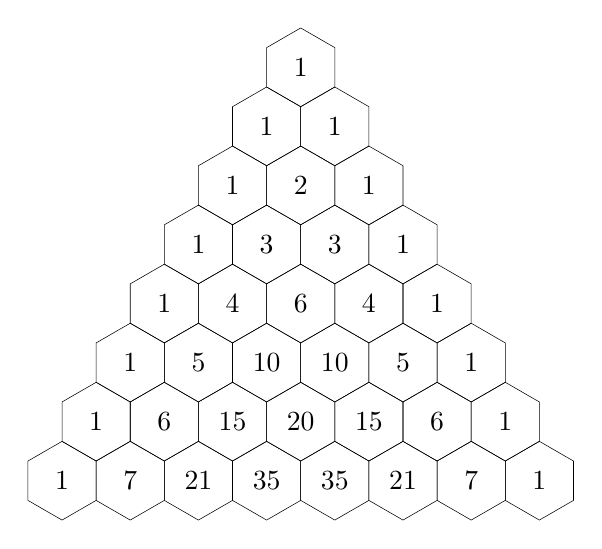
\begin{tikzpicture}
\def\r{.5}
\newcommand{\hexagon}[3]{
  \def\x{-cos{30}*\r*#1+cos{30}*#2*\r*2}
  \def\y{-\r*#1-sin{30}*\r*#1}
  \draw[very thin] (\x,\y) +(90:\r) -- +(30:\r) -- +(-30:\r) -- +(-90:\r) -- +(-150:\r) -- +(150:\r) -- cycle;
  \draw (\x,\y) node{ #3};
}

  
% Pascal's triangle
%put row of 1's down left side:
  \foreach \row in {0,...,7} {
    \hexagon{\row}{0}{ 1}
  }
%fill in the rest of the triangle:
  \foreach \row in {1,...,7} {
    \pgfmathsetmacro{\entry}{1};
    \foreach \col in {1,...,\row} {
      % iterative formula : val = precval * (row-col+1)/col
      % (+ 0.5 to bypass rounding errors)
     \pgfmathtruncatemacro{\entry}{\entry*((\row-\col+1)/\col)+0.5};
      \global\let\entry=\entry
      \ifnum \entry<100
	\hexagon{\row}{\col}{\entry}
      \else \ifnum \entry<1000
	\hexagon{\row}{\col}{\footnotesize \entry}
      \else \ifnum \entry<10000
	\hexagon{\row}{\col}{\footnotesize \entry}
	\else
	\hexagon{\row}{\col}{\scriptsize \entry}
	\fi
      \fi
      \fi
    }
  }
\end{tikzpicture}

\end{center}

There are lots of patterns hidden away in the triangle - enough to fill a reasonably sized book.  Here are just a few of the most obvious ones:
\begin{enumerate}
  \item The entries on the border of the triangle are all 1.
  \item Any entry not on the border is the sum of the two entries above it.
  \item The triangle is symmetric - on any row, entries on the left side are mirrored on the right side.
  \item The sum of all entries on a given row is a power of 2. (You should check this!)
\end{enumerate}

We would like to state these observations in a more precise way, and then prove that they are correct.  Now each entry in Pascal's triangle is in fact a binomial coefficient.  The 1 on the very top of the triangle is ${0 \choose 0}$.  The next row (which we will call row 1, even though it is not the top-most row) consists of ${1 \choose 0}$ and ${1 \choose 1}$.  Row 4 (the row 1, 4, 6, 4, 1) consists of the binomial coefficients
\[{4 \choose 0} ~~ {4 \choose 1} ~~ {4 \choose 2} ~~ {4 \choose 3} ~~ {4 \choose 4}\]
Given this description of the elements in Pascal's triangle, we can rewrite the above observations as follows:
\begin{enumerate}
  \item ${n \choose 0} = 1$ and ${n \choose n} = 1$
  \item ${n \choose k} = {n-1 \choose k-1} + {n-1 \choose k}$
  \item ${n \choose k} = {n \choose n-k}$
  \item ${n\choose 0} + {n \choose 1} + {n \choose 2} + \cdots + {n \choose n} = 2^n$
\end{enumerate}

Each of these are an example of a {\em binomial identity} - a identity (i.e., equation) involving binomial coefficients.

Our goal is to establish these identities - prove that they hold for all values of $n$ and $k$.  These proofs can be done in many ways.  One option would be to give algebraic proofs, using the formula for ${n \choose k}$:
\[{n \choose k} = \frac{n!}{(n-k)!\,k!}\]
Here's how you might do that for the second identity above.

\begin{example}
  Give an algebraic proof for the binomial identity
  \[{n \choose k} = {n-1\choose k-1} + {n-1 \choose k}\]
  \begin{proof}
    By the definition of ${n \choose k}$, we have
    \[{n-1 \choose k-1} = \frac{(n-1)!}{(n-1-(k-1))!(k-1)!} = \frac{(n-1)!}{(n-k)!(k-1)!} \hfill \mbox{ and } {n-1 \choose k} = \frac{(n-1)!}{(n-1-k)!k!}\]
    Thus, starting with the right hand side of the equation we are trying to establish:
    \begin{align*}
      {n-1 \choose k-1} + {n-1 \choose k} & = \frac{(n-1)!}{(n-k)!(k-1)!}+ \frac{(n-1)!}{(n-1-k)!\,k!}\\
      & = \frac{(n-1)!k}{(n-k)!\,k!} + \frac{(n-1)!(n-k)}{(n-k)!\,k!}\\
      & = \frac{(n-1)!(k+n-k)}{(n-k)!\,k!} \\
      & = \frac{n!}{(n-k)!\, k!} \\
      & = {n \choose k}
    \end{align*}
    The second line above (where the common denominator is found) works because $k(k-1)! = k!$ and $(n-k)(n-k-1)! = (n-k)!$.
  \end{proof}

\end{example}

This is certainly a valid proof, but also is entirely useless.  Even if you understand the proof perfectly, it does not tell you {\em why} the identity is true.  In other words, the proof does not have any explanatory power.  A better approach would be to explain what ${n \choose k}$ {\em means} and then say why that is also what ${n-1 \choose k-1} + {n-1 \choose k}$ means.  Let's see how this works for the four identities we have, um, identified.

\begin{example}
  Explain why ${n \choose 0} = 1$ and ${n \choose n} = 1$.
  \begin{solution}
    What do these binomial coefficients tell us? Well, ${n \choose 0}$ gives the number of ways to select 0 objects from a collection of $n$ objects.  There is only one way to do this - to not select any of the objects.  Thus ${n \choose 0} = 1$.  Similarly, ${n \choose n}$ gives the number of ways to select $n$ objects from a collection of $n$ objects.  There is only one way to do this - select all $n$ objects.  Thus ${n \choose n} = 1$.
    
    Alternatively, we know that ${n \choose 0}$ is the number of $n$-bit strings with weight 0 - that is, the number of strings made up of $n$ bits, 0 of which are 1's.  There is only one such string - the string of all 0's.  So ${n \choose 0} = 1$.  Similarly ${n \choose n}$ is the number of $n$-bit strings with weight $n$.  There is only one string - the string of all 1's - with this property.
    
    Another way: ${n \choose 0}$ gives the number of subsets of a set of size $n$ containing 0 elements.  There is only one such subset - the empty set.  ${n \choose n}$ gives the number of subsets containing $n$ elements.  The only such subset is the original set (of all elements).
  \end{solution}

\end{example}

\begin{example}
  Explain why ${n \choose k} = {n-1 \choose k-1} + {n-1 \choose k}$
  \begin{solution}
    The easiest way to see this is to consider bit strings.  ${n \choose k}$ is the number of bit strings of length $n$ containing $k$ 1's.  Of all of these strings, some start with a 1 and the rest start with a 0.  First consider all the bit strings which start with a 1.  After the 1, there must be $n-1$ more bits (to get the total length up to $n$) and exactly $k-1$ of them must be 1's (as we already have one, and we need $k$ total).  How many strings are there like that?  There are exactly ${n-1 \choose k-1}$ such bit strings, so of all the length $n$ bit strings containing $k$ 1's, ${n-1 \choose k-1}$ of them start with a 1.  Similarly, there are ${n-1\choose k}$ which start with a 0 - we still need $n-1$ bits and now $k$ of them must be 1's.  Since there are ${n-1 \choose k}$ bit strings containing $n-1$ bits with $k$ 1's, that is the number of length $n$ bit strings with $k$ 1's which start with a 0.
    
    Another way: consider the question - how many ways can you select $k$ pizza toppings from a menu containing $n$ choices?  One way to do this is just ${n \choose k}$.  Another way to answer the same question is to first decide whether or not you want anchovies.  If you do want anchovies, you still need to pick $k-1$ toppings, now from just $n-1$ choices.  That can be done in ${n-1 \choose k-1}$ ways.  If you do not want anchovies, then you still need to select $k$ toppings from $n-1$ choices (the anchovies are out).  You can do that in ${n-1 \choose k}$ ways.  Since the choices with anchovies are disjoint from the choices without anchovies, the total choices are ${n-1 \choose k-1}+{n-1 \choose k}$.  But wait.  We answered the same question in two different ways - so the two answers must be the same.  Thus ${n \choose k} = {n-1\choose k-1} + {n-1 \choose k}$.
    
    You can also explain (prove) this identity by counting subsets, or even lattice paths.
  \end{solution}

\end{example}


\begin{example}
  Prove the binomial identity ${n \choose k} = {n \choose n-k}$.
  \begin{solution}
    Why is this true?  ${n \choose k}$ counts the number of ways to select $k$ things from $n$ choices.  On the other hand, ${n \choose n-k}$ counts the number of ways to select $n-k$ things from $n$ choices.  Are these really the same?  Well, what if instead of selecting the $n-k$ things you choose to exclude them.  How many ways are there to choose $n-k$ things to exclude from $n$ choices.  Clearly this is ${n \choose n-k}$ as well (it doesn't matter whether you include or exclude the things once you have chosen them).  And if you exclude $n-k$ things, then you are including the other $n$ things.  So the set of outcomes should be the same.
    
    Let's do the pizza counting example like we did above.  How many ways are there to pick $k$ toppings from a list of $n$ choices?  On the one hand, then answer is simply ${n \choose k}$.  Alternatively, you could make a list of all the toppings you don't want.  To end up with a pizza containing exactly $k$ toppings, you need to pick $n-k$ toppings to not put on the pizza.  You have ${n \choose n-k}$ choices for the toppings you don't want. Both of these ways give you a pizza with $k$ toppings - in fact all the ways to get a pizza with $k$ toppings.  Thus  these two answers must be the same: ${n \choose k} = {n \choose k-1}$.
    
    You can also prove (explain) this identity using bit strings, subsets, or lattice paths.  The bit string argument is nice: ${n \choose k}$ counts the number of bit strings of length $n$ with $k$ 1's.  This is also the number of bit string of length $n$ with $k$ 0's though - just replace each 1 with a 0 and each 0 with a 1.  But if a string of length $n$ has $k$ 0's, it must have $n-k$ 1's.  And there are exactly ${n\choose n-k}$ strings of length $n$ with $n-k$ 1's.
  \end{solution}
\end{example}

\begin{example}
  Prove the binomial identity ${n\choose 0} + {n \choose 1} + {n\choose 2} + \cdots + {n \choose n} = 2^n$
  \begin{solution}
    Let's do a ``pizza proof'' again.  We need to find a question about pizza toppings which has $2^n$ as the answer.  How about this: If a pizza joint offers $n$ toppings, how many pizzas can you build using any number of toppings from no toppings to all toppings, using each topping at most once?
    
    On one hand, the answer is $2^n$ - for each topping you can say ``yes'' or ``no,'' so you have two choices for each topping.
    
    On the other hand, divide the possible pizzas into disjoint groups - the pizzas with no toppings, the pizzas with one topping, the pizzas with two toppings, etc.  If we want no toppings, there is only one pizza like that (the empty pizza, if you will) but it would be better to think of that number as ${n \choose 0}$ - we choose 0 of the $n$ toppings.  How many pizzas have 1 topping?  We need to choose 1 of the $n$ toppings, so ${n \choose 1}$.  We have:
    \begin{itemize}
      \item[] Pizzas with 0 toppings: ${n \choose 0}$
      \item[] Pizzas with 1 topping: ${n \choose 1}$
      \item[] Pizzas with 2 toppings: ${n \choose 2}$
      \item[$\vdots$] ~
      \item[] Pizzas with $n$ toppings: ${n \choose n}$.
    \end{itemize}
    The total number of possible pizzas will be the sum of these, which is exactly the left hand side of the identity we are trying to prove.  
    
    Again, we could have proved the identity using subsets, bit strings, or lattice paths (although the lattice path argument is a little tricky). 
  \end{solution}

\end{example}

Hopefully this gives some idea of how explanatory proofs of binomial identities can go.  It is worth pointing out that sometimes more traditional proofs are also nice.\footnote{Most every binomial identity can be proved using mathematical induction, using the recursive definition for ${n \choose k}$.  We will discuss induction later in the course.}  For example, consider the following rather slick proof of the last identity.

Recall the binomial theorem:
\[(x + y)^n = {n \choose 0}x^n + {n \choose 1}x^{n-1}y + {n \choose 2}x^{n-2}y^2 + \cdots + {n \choose n-1}x\cdot y^n + {n \choose n}y^n\]
Let $x = 1$ and $y = 1$.  We get:
\[(1 + 1)^n = {n \choose 0}1^n + {n \choose 1}1^{n-1}1 + {n \choose 2}1^{n-2}1^2 + \cdots + {n \choose n-1}1\cdot 1^n + {n \choose n}1^n\]
Of course this simplifies to:
\[(2)^n = {n \choose 0} + {n \choose 1} + {n \choose 2} + \cdots + {n \choose n-1} + {n \choose n}\]
Something fun to try: Let $x = 1$ and $y = 2$.  Neat huh?

\subsection{More Proofs}

The explanatory proofs given in the above examples are typically called {\em combinatorial proofs}.  In general, to give a combinatorial proof for a binomial identity, say $A = B$ you do the following:
\begin{enumerate}
  \item Find a counting problem you will be able to answer in two ways.
  \item Explain why one answer to the counting problem is $A$.
  \item Explain why the other answer to the counting problem is $B$.
\end{enumerate}

Since both $A$ and $B$ are the answers to the same question, we must have $A = B$.  

The tricky thing is coming up with the question.  This is not always obvious, but it gets easier the more counting problems you solve.  You will start to recognize types of answers as the answers to types of questions.  More often what will happen is you will be solving a counting problem and happen to think up two different ways of finding the answer.  Now you have a binomial identity and the proof is right there - the proof {\em is} the problem you just solved together with your two solutions.

For example, consider this counting question:

\begin{quote}
  How many 10-letter words contain exactly four A's, three B's, two C's and one D?
\end{quote}

Let's try to solve this problem.  We have 10 spots for letters to go.  Four of those need to be A's.  We can pick the four A-spots in ${10 \choose 4}$ ways.  Now where can we put the B's?  Well there are only 6 spots left, we need to pick $3$ of them.  This can be done in ${6 \choose 3}$ ways.  The two C's need to go in two of the 3 remaining spots, so we have ${3 \choose 2}$ ways of doing that.  That leaves just one spot of the D, but we could write that 1 choice as ${1 \choose 1}$.  Thus the answer is:
\[{10 \choose 4}{6 \choose 3}{3 \choose 2}{1 \choose 1}\]
But why stop there?  We can find the answer another way too.  First let's decide where to put the one D: we have 10 spots, we need to choose 1 of them, so this can be done in ${10 \choose 1}$ ways.  Next, choose one of the ${9 \choose 2}$ ways to place the two C's.  We now have $7$ spots left, and three of them need to be filled with B's.  There are ${7 \choose 3}$ ways to do this.  Finally the A's can be placed in ${4 \choose 4}$ (that is, only one) ways.  So another answer to the question is
\[{10 \choose 1}{9 \choose 2}{7 \choose 3}{4 \choose 4}\]
Interesting.  This gives us the binomial identity:
\[{10 \choose 4}{6 \choose 3}{3 \choose 2}{1 \choose 1} = {10 \choose 1}{9 \choose 2}{7 \choose 3}{4 \choose 4}\]
Here are a couple of other binomial identities with combinatorial proofs.

\begin{example}
  Prove the identity
  \[1 n + 2(n-1) + 3  (n-2) + \cdots + (n-1) 2 + n  1 = {n+2 \choose 3}\]
  \begin{solution}
    To give a combinatorial proof we need to think up a question we can answer in two ways: one way needs to give the left-hand-side of the identity, the other way needs to be the right-hand-side of the identity.  Our clue to what question to ask comes from the right hand side: ${n+2 \choose 3}$ counts the number of ways to select 3 things from a group of $n+2$ things.  Let's name those things $1, 2, 3, \ldots, n+2$.  In other words, we want to find 3-element subsets of those numbers (since order should not matter, subsets are exactly the right thing to think about).  We will have to be a bit clever to explain why the left-hand-side also gives the number of these subsets.  Here's the proof.
    
    \begin{proof}
      Consider the question ``How many 3-element subsets are there of the set $\{1,2,3,\ldots, n+2\}$?''  We answer this in two ways:
      
      \underline{Answer 1}: We must select 3 elements from the collection of $n+2$ elements.  This can be done in ${n+2 \choose 3}$ ways.
      
      \underline{Answer 2}: Break this problem up into cases, by what the middle number in the subset is.  That is, each subset is $\{a,b,c\}$, say written in increasing order.  We count how many such subsets there are for each distinct value of $b$.  The smallest possible value of $b$ is $2$, and the largest is $n+1$.  
      
      When $b = 2$, there are $1 \cdot n$ subsets - 1 choice $a$ and $n$ choices (3 through $n+2$) for $c$.
      
      When $b = 3$, there are $2 \cdot (n-1)$ subsets - 2 choices for $a$ and $n-1$ choices for $c$.
      
      When $b = 4$, there are $3 \cdot (n-2)$ subsets - 3 choices for $a$ and $n-2$ choices for $c$.
      
      And so on.  When $b = n+1$, there are $n$ choices for $a$ and only 1 choice for $c$, so $n \cdot 1$ subsets.
      
      Therefore the total number of subsets is \[1 n + 2 (n-1) + 3  (n-2) + \cdots + (n-1)2 + n  1.\]
      
      Since Answer 1 and Answer 2 are answers to the same question, they must be equal.  Therefore
      \[1 n + 2 (n-1) + 3  (n-2) + \cdots + (n-1) 2 + n  1 = {n+2 \choose 3}\]
      
    \end{proof}

  \end{solution}

\end{example}


\begin{example}
  Prove the binomial identity
  \[{n \choose 0}^2 + {n \choose 1}^2 + {n \choose 2}^2 + \cdots + {n \choose n}^2 = {2n \choose n}\]
  \begin{solution}
    We will give two different proofs of this fact.  The first will be very similar to the previous example (counting subsets).  The second proof is a little slicker - it will use lattice paths.
    
    \begin{proof}
      Consider the question: ``How many pizzas can you make using $n$ toppings when there are $2n$ toppings to choose from?''
      
      \underline{Answer 1}:  There are $2n$ toppings, from which you must choose $n$.  This can be done in ${2n \choose n}$ ways.
      
      \underline{Answer 2}: Divide the toppings into two groups of $n$ toppings (perhaps $n$ meats and $n$ veggies).  Any choice of $n$ toppings must include some number from the first group and some number from the second group.  Consider each possible number of meat toppings separately:
      
      0 meats: ${n \choose 0}{n \choose n}$, since you need to choose 0 of the $n$ meats and $n$ of the $n$ veggies.
      
      1 meat: ${n \choose 1}{n \choose n-1}$, since you need 1 of $n$ meats so $n-1$ of $n$ veggies.
      
      2 meats: ${n \choose 2}{n \choose n-2}$.  Choose 2 meats and the remaining $n-2$ toppings from the $n$ veggies.
      
      And so on.  The last case is $n$ meats, which can be done in ${n \choose n}{n \choose 0}$ ways.
      
      Thus the total number of pizzas possible is
      \[{n \choose 0}{n \choose n} + {n \choose 1}{n \choose n-1} + {n \choose 2}{n \choose n-2} + \cdots + {n \choose n}{n \choose 0}\]
      This is not quite the left hand side \ldots yet.  Notice that ${n \choose n} = {n \choose 0}$ and ${n \choose n-1} = {n  \choose 1}$ and so on, by the symmetry formula.  Thus we do indeed get
      \[{n \choose 0}^2 + {n \choose 1}^2 + {n \choose 2}^2 + \cdots + {n \choose n}^2\]      
    \end{proof}
    
    Here's the second proof:
    
    \begin{proof}
      Consider the question: ``How many lattice paths are there from $(0,0)$ to $(n,n)$?''
      
      \underline{Answer 1}: We must travel $2n$ units, and $n$ of them must be in the up direction.  Thus there are ${2n \choose n}$ paths.
      
      \underline{Answer 2}: Note that any path from $(0,0)$ to $(n,n)$ must cross the line $x + y = n$.  That is, must pass through exactly one of the points: $(0,n)$, $(1,n-1)$, $(2,n-2)$, \ldots, $(n, 0)$.  For example, this is what happens in the case $n = 4$:
        
    \begin{center}
    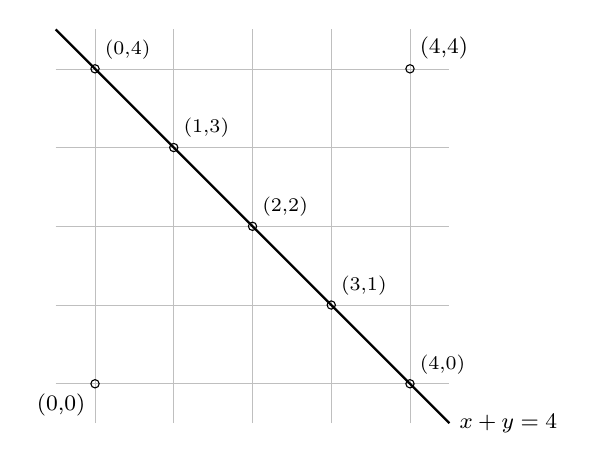
\begin{tikzpicture}
      \draw[very thin, color=gray!50] (-.5,-.5) grid (4.5, 4.5);
%       \foreach \x in {0,...,4}
%       \foreach \y in {0,...,4}
%       \fill (\x,\y) circle (1.5pt);
      \draw (0,0) circle (1.5pt) node[below left] {\footnotesize (0,0)} (4,4) circle (1.5pt) node[above right] {\footnotesize (4,4)};
      \draw[thick] (-.5, 4.5) -- (4.5, -.5) node[right]{\footnotesize $x + y = 4$};
      \draw (0,4) circle (1.5pt) node[above right]{\scriptsize (0,4)} (1,3) circle (1.5pt) node[above right]{\scriptsize (1,3)} (2,2) circle (1.5pt) node[above right]{\scriptsize (2,2)} (3,1) circle (1.5pt) node[above right]{\scriptsize (3,1)} (4,0) circle (1.5pt) node[above right]{\scriptsize (4,0)}; 
    \end{tikzpicture}
   \end{center}
     
     How many paths pass through $(0,n)$?  To get to that point, you must travel $n$ units, and $0$ of them are to the right, so there are ${n \choose 0}$ ways to get to $(0,n)$.  From $(0,n)$ to $(n,n)$ takes $n$ steps, and $0$ of them are up.  So there are ${n \choose 0}$ ways to get from $(0,n)$ to $(n,n)$.  Therefore there are ${n \choose 0}{n \choose 0}$ paths from $(0,0)$ to $(n,n)$ through the point $(0,n)$.  
     
     What about through $(1,n-1)$.  There are ${n \choose 1}$ paths to get there ($n$ steps, 1 to the right) and ${n \choose 1}$ paths to complete the journey to $(n,n)$ ($n$ steps, $1$ up).  So there are ${n \choose 1}{n \choose 1}$ paths from $(0,0)$ to $(n,n)$ through $(1,n-1)$.
     
     In general, to get to $(n,n)$ through the point $(k,n-k)$ we have ${n \choose k}$ paths to the mid point and then ${n \choose k}$ paths from the mid point to $(n,n)$.  So there are ${n \choose k}{n \choose k}$ paths from $(0,0)$ to $(n,n)$ through $(k, n-k)$.
     
     All together then the total paths from $(0,0)$ to $(n,n)$ passing through exactly one of these mid points is
     \[{n \choose 0}^2 + {n \choose 1}^2 + {n \choose 2}^2 + \cdots + {n \choose n}^2\]      
   \end{proof}
  \end{solution}
\end{example}



\end{document}


